When simulating physical phenomena one must choose a model which fits
the phenomena being modeled. The level set method (LSM), is a method
for modelling phenomena that can be described in terms of moving level
sets.
%
A level set in it self is only a mathematical function that groups
variables which have the same function value. It describes a
parametric function in one dimension higher than its original domain,
gaining the ability to describe more than one not colocated level set
in the same structure.
%
A two dimensional level set is known as a level curve or isocontour,
which uses two dimensions to describe curves. We encounter isocontours
in everyday life as pressure information in the weather cast and
terrain elevation on maps.
%
A three dimensional level set is
known as a level surface or isosurface, and is used, as suggested be
it's name, to describe surfaces.  A general a level set in n
dimensions is used to describe n-1 dimensional objects. Mathematically
a level set is define as follows:

\begin{equation}
\{ (x_1,...,x_n) \} | f(x_1,...,x_n) = c
\end{equation}

In words this means that all values of $v_i$ leading to a function
value of $c$ defines the level set $c$.
%
The level set in it's own right does not make a simulation. Unless it
is evolved over times it stays the same. To evolve the level set over
time partiel differential equations (PDEs) describing the physical
phenomena needs to be solved to move the level sets.
%
Typical phenomena modeled by the LSM includes: computational fluid
dynamics (CFG), and fire and explosion simulation. \todo{more examples
please}

In this report, we will explain what the Level Set method is and what
its applications are. Furthermore, we will provide code examples of
how to implement the mathematical formulas needed to create a Level
Set framework.

The Level Set method is a numerical technique used to move
surfaces. The surfaces are moved by solving a partial differential
equation(PDE) dependant on a time factor.

In figure \vref{fig:heightmap} we see two figures describing a 2-d and
3-d view of an island. Figure \vref{fig:isocontour-2d} describes an
isocontour map of heights where the color indicates the height of each
point. The brighter the color the higher the point. Figure
\vref{fig:isocontour-3d} shows the corresponding 3d view.

\begin{figure}[h]
\begin{center}
  \subfloat[2D view of an elevation isocontour map]{
    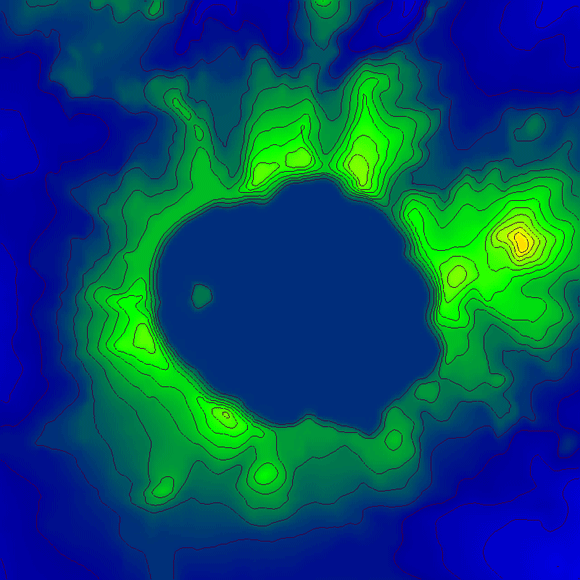
\includegraphics[width=0.5\textwidth]{imgs/226171_226171.png}
    \label{fig:isocontour-2d}
  }
  \subfloat[3D view of figure \ref{fig:isocontour-2d}]{
    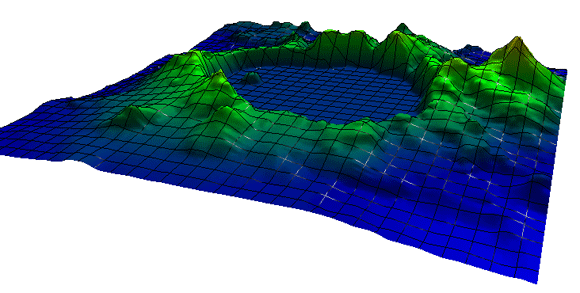
\includegraphics[width=0.5\textwidth]{imgs/226170_226170.png}
    \label{fig:isocontour-3d}
  }
\end{center}
\caption{Illustrations of heightmap, from: Intel Array Visualizer
  Gallery, \cit{intel}}
\label{fig:heightmap}
\end{figure}


\todoHave{husk reference}

%\image{hoejdekort.png}{0.25}{A topographic map indicating heights in the vermont region.}{introduction:fig:hoejdekort}

For a level set representation there is an underlying function
describing the topology. Each contour corresponds to a set of points
in this function with the same value, thus we need a function which
produces a field of values. In heightmaps, it would be a function from
$(x,y)$ coordinates to a height. In general, any function producing a
field of values is sufficient.  

One function that has the desired characteristics is a function known
as the signed distance function $\phi$.

\section*{Signed distance function - $\phi$}

In a level set context, the signed distance function is essentially a
measure of, for each point in the domain how far that point is from
the zero isocontour.

Since this function produces the straightforward euclidian distance,
it increases linearly. 

In order to use an implicit representation of the surface we use a
signed distance field as the underlying function to the level set. We
define the zero isocontour of this function to be the surface.

The Level Set method can use implicit functions which means that the
function is defined in the entire plane and not only on the surface.

The function $\phi(x,y)$ is a signed distance function in all of
$\mathbb{R}^{n}$, in our case $\mathbb{R}^{2}$. A signed distance
function $\phi$ is a function that given a point on the plane, returns
the distance to the surface. We have that $\phi(x,y) > 0$ if we are
outside the object and $\phi(x,y) < 0$ when we are inside the object.
And last, when $\phi(x,y) = 0$ we are on the interface or iso-surface.
The iso-surface separates the inside and outside.  Besides indicating
whether we are inside or outside an object, it also indicates how far
we are from the closest point on the iso-surface which is quite
handy. For a picture of the above, see figure
\vref{introduction:fig:implicitfunction}.

\image{phi.png}{0.3}{The figure is borrowed from
\cit{osher2002level}. A implicit function, defined in all of
$\mathbb{R}^{2}$. We see that when we are inside the object then
$\phi$ is less than zero, larger when we are outside and zero on the
interface.}{introduction:fig:implicitfunction}\todoPtx{Man kunne lave
mere vektor grafik her, fx. med cirklen i stedet.}

%% Example - Circle

\subsection*{Example}

A simple example is to consider a circle and its equation:
\begin{equation*} 
  x^{2} + y^{2} = r^{2}
\end{equation*}

It is defined in all points in $\mathbb{R}^{2}$ and is an example of
an implicit function. Given a specific radius $r$, the equation of a
circle defines an isocontour. If $r = 5$, then the isovalue is $c =
5^{2} = 25$. For all the points $(x,y)$ that evaluate to 25 gives us
the isosurface. If the value is smaller then it is inside the surface,
and outside when the value is greater. See figure
\vref{introduction:fig:cartesiangrid}.


\section*{Cartesian grid}
\begin{comment} Finite memory -> descritization of plane -> cartesian
grid is used.
\end{comment}

Since a computer has finite memory we need to come up with a way to
store our representation. A simple way to do this is to partition the region into a grid where each
square is of equal size. Normally

\begin{figure}[htb] \centering
    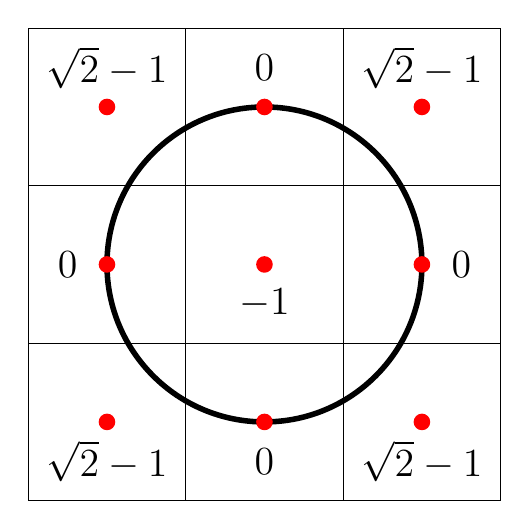
\begin{tikzpicture}[font=\Large]
    \draw (0,0) rectangle +(2,2)
    +(1,0.5) node {$-1$};    
    \draw (0,2) rectangle +(2,2)
    +(1,1.5) node {$0$};
    \draw (2,0) rectangle +(2,2)
    +(1.5,1) node {$0$};
    \draw (0,-2) rectangle +(2,2)
    +(1,0.5) node {$0$};
    \draw (-2,0) rectangle +(2,2)
    +(0.5,1) node {$0$};
    \draw (2,2) rectangle +(2,2)
    +(1,1.5) node {$\sqrt{2}-1$};
    \draw (2,-2) rectangle +(2,2)
    +(1,0.5) node {$\sqrt{2}-1$};
    \draw (-2,2) rectangle +(2,2)
    +(1,1.5) node {$\sqrt{2}-1$};
    \draw (-2,-2) rectangle +(2,2)
    +(1,.5) node {$\sqrt{2}-1$};
    \draw[line width=2pt] (1,1) circle (2);
    \fill[shift={(1,1)},red]
    (0,0) circle (3pt)
    (2,0) circle (3pt)
    (0,2) circle (3pt)
    (-2,0) circle (3pt)
    (0,-2) circle (3pt)
    (-2,-2) circle (3pt)
    (2,-2) circle (3pt)
    (-2,2) circle (3pt)
    (2,2) circle (3pt)    
    ;
  \end{tikzpicture}
  \caption{A circle, descritized into a cartesian grid. The value in
    each cell is the $\phi$ value described in this chapter.}
  \label{introduction:fig:cartesiangrid}
\end{figure}

In figure \vref{introduction:fig:cartesiangrid}, we see how a plane
has been descritized into a cartesian grid, showing a circle and the
values of $\phi$.

%% formulas

\section*{Solving the Level Set}\label{sec:intro:solve} 

\todoPtx{I own this!!}

If we want to move the level set, we have to iteratively solve a
Partial differential equation to make the surface move. We solve a
partial differential equation in all points $(x,y) | x,y \in
\mathbb{R}^{2}$. If we want to move the interface in the normal
direction we solve the following equation:

\begin{equation}
\phi_{t} + a|\nabla \phi| = 0
\end{equation}\label{eq:normMove}

where $\nabla \phi = (\dfrac{\partial \phi}{\partial x},
\dfrac{\partial \phi}{\partial y})$ and $a$ can be of either sign.

When $a > 0$ the interface moves in the normal direction and when $a <
0$ it moves in the opposite direction of the normal.


\section*{Applications}

The advantages are that since we discretize the surface into a
cartesian grid, we can do numerical computations without having to
parameterize the objects. Another advantage is that the level set
method makes it easy to work on geometry that change topology over
time.


%% applications.  So why do we want to use the level set method? A
simple example is to consider an object that splits in two or two
objects merging into one. If we did not use the level set method, we
would have to explicitely represent the two new objects, where in the
level set case we get this for free do to the implicit representation.

\todoPtx{måske lidt flere anvendelsesmuligheder (lysberegninger her!)}

\newpage

\section*{Outline of the report}\todoPtx{Denne er på en side for sige
selv, så vref ikke crasher}

In chapter \vref{chap:sdf}, we give an in depth look on the signed
distance function, describe what kinds of mathematical operations we
have in our toolbox and describe the important reinitialize function,
section \vref{sec:reinitialize}.

In chapter \vref{chap:extensions}, we look at extension that can be
made to the basic level set implementation that we have done. In
section \vref{sec:segmentation}, we look at how to implement
segmentation algorithms which can be used in mediacal imaging. In
section \vref{sec:fluid}, we implement a fluid solver for computer
graphics using the level set method. And finally, in section
\vref{sec:imagereconstruction} \todoHave{Skal CPVC's afsnit være med i
den endelige rapport? (have)} we use the level set to do computations
on images.



%%% Local Variables: 
%%% mode: latex 
%%% mode: auto-fill 
%%% TeX-PDF-mode: t 
%%% TeX-master: "../master.tex" 
%%% End:

